%\documentclass[twocolumn]{IEEEtran}
%\documentclass[onecolumn]{IEEEtran}
\documentclass[journal,10pt]{IEEEtran}
\usepackage{graphicx}
%%%\usepackage{caption}
%\usepackage[numbers]{natbib}
%\usepackage[sort,numbers]{natbib}
\usepackage{verbatim}
\usepackage{subcaption}
\usepackage[nocompress]{cite}
\usepackage{amsmath, amsthm, amssymb}
\usepackage{enumerate}
\usepackage{url}
\usepackage{epstopdf}
\newtheorem{theorem}{Theorem}
\newtheorem{lemma}{Lemma}
\newtheorem{definition}{\bf Definition}
\newtheorem{remark}{Remark}
\theoremstyle{definition}
\newtheorem{example}{Example}
\usepackage{extarrows}
\usepackage{amsfonts}
\usepackage{algorithm, algorithmic}
\usepackage{color}
\usepackage{mathrsfs}
\usepackage{multirow}
\usepackage{amsmath}
\usepackage{cases}
\usepackage{hyperref} %������
\hypersetup{%hypertex=true,
            colorlinks=true,
            linkcolor=black,
            anchorcolor=blue,
            citecolor=black}
\title{Robust Power Control and Task Offloading for Cloud Assisted MEC in Vehicular Networks}
\newcommand{\mykeywords}{Internet of Vehicle (IoV), Computation Offloading, Robust Power Control, Edge Computing, Bernstein Method} %
\makeatletter
\newcommand{\ALOOP}[1]{\ALC@it\algorithmicloop\ #1
  \begin{ALC@loop}}
\newcommand{\ENDALOOP}{\end{ALC@loop}\ALC@it\algorithmicendloop}
\renewcommand{\algorithmicrequire}{\textbf{Input:}}
\renewcommand{\algorithmicensure}{\textbf{Output:}}
\newcommand{\algorithmicbreak}{\textbf{break}}
\newcommand{\BREAK}{\STATE \algorithmicbreak}
%%%%%%\hypersetup{pdftitle={\@title},pdfauthor={Zhixin Liu},pdfkeywords={\mykeywords},pdfsubject={ },pdfproducer={ }} % ����PDF��ProducerԪ���� ���� ������}  ,pdfauthor={\@author}   ,pdfproducer={}
\makeatother
% *** GRAPHICS RELATED PACKAGES ***
\ifCLASSINFOpdf
\else
\fi
\hyphenation{op-tical net-works semi-conduc-tor}
\begin{document}
%\begin{comment}
\author{Zhixin Liu, % ~\IEEEmembership{Senior Member,~IEEE},
 Jianshuai Wei, Jiawei Su, Kit Yan Chan,  Yazhou Yuan%, and Xinping Guan, ~\IEEEmembership{Fellow,~IEEE}
%
\thanks{Zhixin Liu, Jianshuai Wei, Jiawei Su and Yazhou Yuan
are with the School of Electrical Engineering, Yanshan
University, Qinhuangdao 066004, China. Emails: lzxauto@ysu.edu.cn,
jswe@stumail.ysu.edu.cn, Sjw@stumail.ysu.edu.cn, yzyuan@ysu.edu.cn.}
\thanks{Kit Yan Chan is with the School of Electrical Engineering, Computing and Mathematical Sciences, Curtin University, Perth, Australia. Email: kit.chan@curtin.edu.au.}
%\thanks{Xinping Guan is with the School of Electronic, Information and Electrical Engineering, Shanghai Jiaotong University, Shanghai 200240, China. Email: xpguan@sjtu.edu.cn.}
\thanks{This work is supported partly by National Natural Science Foundation of China under Grant 62273298, 62273295.}}

%\end{comment}
\markboth{MANUSCRIPT}{}
\maketitle
\begin{abstract}
\begin{comment}
Cloud-assisted mobile-edge computing (C-MEC) has emerged as a promising solution for task offloading in vehicular networks, offering abundant computing resources. In this paper, a robust power control and task offloading scheme is proposed to offload the computation task and maximize the utility of C-MEC networks. However, an uncertain channel state influences the stability of transmitting the offloading task significantly. In order to simulate channel uncertainty, a first-order Markov process is adopted, where the vehicular mobility is considered. Moreover, channel reusing is assumed to be caused by the limited spectrum resources which leads to complex co-channel interference. To overcome the limitations, probability constraints of signal links are enforced to ensure communication quality. A Bernstein approximations method is adopted to transform the original constraints into solvable constraints. Scrupulously, the block coordinate descent (BCD) method and the successive convex approximation (SCA) technique are further adopted to solve the nonconvex robust optimization problem. A robust power control and task offloading scheduling algorithm is proposed to determine the optimal solutions. The proposed algorithm undergoes numerical simulations to evaluate the performance of the system. The obtained results demonstrate its effectiveness compared to benchmark models, particularly in communication environments with channel uncertainty.
\end{comment}
Cloud-assisted mobile-edge computing (C-MEC) is a promising solution for task offloading in vehicular networks, providing abundant computational resources. This paper proposes a robust power control and task offloading scheme to maximize the utility of C-MEC networks. However, an uncertain channel state significantly affects the stability of the offload task transmission. Additionally, channel reuse is assumed to be a result of limited spectrum resources, leading to complex co-channel interference. The objective function is a non-convex form that is challenging to solve. To simulate channel uncertainty, a first-order Markov process is adopted, taking into account vehicle mobility. To address co-channel interference limitations, probability constraints on signal links are enforced to ensure communication quality. A Bernstein approximation method is employed to transform the original constraints into solvable ones. The Block Coordinate Descent (BCD) method and the Successive Convex Approximation (SCA) technique are scrupulously applied to solve the non-convex robust optimization problem. A robust power control and task offloading scheduling algorithm is proposed to determine optimal solutions. Numerical simulations are conducted to evaluate the system's performance. The results indicate its effectiveness compared to benchmark models, particularly in communication environments with channel uncertainty.
\end{abstract}
\begin{IEEEkeywords}
\mykeywords
\end{IEEEkeywords}
\section{Introduction} \label{introduction}
\begin{comment}
Mobile-edge computing (MEC) and mobile cloud computing (MCC), as two new architectures for the
emerging 5G networks, are commonly used to support task offloading for Internet of Things devices,
especially providing the low-latency and high-reliability computing services \cite{sym2019},\cite{Ramesh2023}. At the edge of the network center, MEC reduces transmission delay and allocates computing resources to vehicles to relieve the computational pressures \cite{Wang2020}.
\end{comment}
Mobile Edge Computing (MEC) and Mobile Cloud Computing (MCC) are two emerging architectures for 5G networks that support task offloading for Internet of Things devices. MEC acts as a cloud service provider at the edge of the network, providing storage, image caching, and third-party access capabilities. This reduces bandwidth pressure on the wireless network and provides low-latency and high-reliability computing services. %\cite{sym2019},
\cite{Ramesh2023}. MEC also reduces the transmission delay and allocates computational resources to vehicles to relieve the computational pressure \cite{Wang2020}. MEC plays an important role in providing intelligent traffic identification and control, which enables the disaggregation of the mobile network.However, the computing resources of MEC are still insufficient when the computing tasks are demanding. Since high-performance computing is provided by cloud servers, cloud-based computing networks have been deployed to meet the exploding demand for computation offloading. However, cloud computing centers tend to be far from the main roads, resulting in long latency for cloud computing \cite{Qian2023}. In the highly dynamic Internet of Vehicles, the data transmitted by vehicles must be processed in real time \cite{Pang2021}. Therefore, the cloud-assisted mobile-edge computing (C-MEC) is used for the network architecture to provide rich computing resources and reduce the transmission latency.

However, past experience has shown that interference in the dynamic vehicle scenario often results in significantly degraded quality of service (QoS) for communication in current mobile edge computing, which enables vehicular networks \cite{Guan2023}. In addition, vehicle mobility causes an uncertain channel state and it further significantly affects and destabilizes the communication quality.
By deploying joint power control and computing resource allocation in the multi-vehicles in multi-MEC systems will solve the task offloading problem in a C-MEC vehicular network and will guarantee the QoS.
\subsection{Related Works}
Recently, some research has been conducted to improve the effectiveness and robustness of Internet of Vehicle (IoV) edge computing networks, which consist of cloud computing layers and MEC layer vehicle network architectures. Zhou et al. \cite{Zhou2019} proposed a computing framework for vehicular networks with a hierarchical structure, which is composed of the control layer, the vehicular edge computing server layer, and the vehicular network layer. Dai et al. \cite{Dai2022} conducted research on enhancing the cooperative computation offloading service in MEC-assisted service architecture, where multiple MEC servers and remote cloud offloading of computation-intensive tasks are implemented collaboratively. Some research proposed methods to improve computation offloading performance in the C-MEC vehicular network scenario. Tan and Hu \cite{Tan2018} have formulated and solved the joint communication, caching, and computing problem in order to optimize the operational excellence and cost efficiency of vehicular networks. Wang et al. \cite{Wang2020} formulated the problem as a generalized NE problem and proposed a game theory algorithm to analyze the equilibrium problem. Wang et al. \cite{Wang2022} developed a distributed clustering mechanism that organizes vehicles into several cooperative edge servers to optimize total revenue during the entire scheduling process. Li et al. \cite{Li2023} developed an analytical model of the service cache at the edge of the vehicle, mainly considering the offloading of computational tasks and task interdependence between Roadside Units (RSUs). However, the aforementioned methods only optimized one of the two indices, power control and computing resource allocation. Some research assumed that the vehicles maintain constant transmit power. Our approach takes a multifaceted approach toward optimization, which includes optimizing both the vehicle's transmit power and the computational resource allocation for a multivehicle and mult-MEC server system. A new challenge is created since the objective function is difficult to optimize. A convex approximation approach for optimizing the objective function has been suggested by Nemirovski and Shapiro \cite{Nemirovski2007}. To solve non-convex problems with two variables, some research decouples the original problem into two sub-problems, and the Block Coordinate Descent (BCD) method is employed to address the two sub-problems.

Unlike traditional mobile communication networks with low mobility, the Doppler effect in highly mobile vehicles poses a challenge to C-MEC communication when fast-moving vehicles communicate with different MEC servers. Deterministic channel state information (CSI) is no longer sufficient to describe the channel state in network scenarios with dynamic characteristics. The Doppler effect created during transmission significantly impacts the small-scale fading of CSI, resulting in fast channel variations. In other words, the used CSIs are outdated. To depict the effects of Doppler frequency shift on the channel, the First-order Gauss-Markov process is utilized \cite{Liu2019}. To improve performance with low communication and computing delays, vehicle equipment has a reduced tolerance for delay and transmission reliability. Therefore, higher requirements are essential. In \cite{Li2020}, Li et al. introduced an outage probability constraint to ensure the reliability of vehicular communication links. When the exact expression includes the exponential integral function, it is necessary to consider an approximate closed-form expression to make it tractable and reduce the computational complexity.

In C-MEC vehicular networks, authorized vehicles with spectrum resources directly communicate with RSU. However, scarce spectrum resources are inadequate in high-density vehicular networks \cite{Xie2020}. Zhou et al. \cite{Zhou2017} developed a dynamic sharing approach for 5G spectrums, and they proposed a sharing architecture of Dedicated Short Range Communications (DSRC) and the 5G spectrum to enable immersive experience-driven vehicular communications. Tran et al. \cite{Tran2019} proposed a comprehensive approach to tackle the challenge of task offloading and resource allocation in a multi-server MEC-assisted network. The results showed that effective channel reusing is crucial when the spectrum resources are scarce \cite{Liang2021}. However, the approach generally creates interference, where the interference caused by channel reuse in the vehicle communication scenario often degrades communication quality sharply. To deal with the outage probability constraint, Xiao et al. \cite{Xiao2020} assumed that the CSIs can be obtained by estimation. Therefore, the outage constraint is transformed into the Bernstein-type inequality to formulate the deterministic optimization problem \cite{Chen2022}.
To simulate the interference constraint, the probability constraints are introduced to resolve the uncertain co-channel interference, and the Bernstein approximation method is used to transform the interference constraint into a solvable closed form. The method has been widely used to solve the hard non-convex problems \cite{Wang2015}. Describing the dynamic topology of vehicle networks by the probabilistic constraints can improve QoS.
Additionally, the paper employs the Bernstein method because of the uncertain constraint characteristics. In summary, existing research has tackled power control and computing resource allocation problems, which assists MEC in vehicular networks in highly dynamic environments. %Also, no research attempts to ensure communication quality and latency requirements are satisfactory.
\subsection{Contributions}
In this paper, a robust power control and task offloading algorithm is proposed for the cloud to assist MEC in vehicular networks with highly dynamic vehicles. Unlike the existing unilateral research on power control or resource allocation computation, a network system that heavily emphasizes collaboration is investigated, and the communication delay and computing delay are guaranteed by satisfying the probabilistic constraints. The framework also guarantees vehicle QoS. To summarize, this paper's primary contributions can be outlined as follows:

\begin{itemize}

  \item The practical C-MEC vehicular networks for computation offloading architecture is considered. Since the MEC layer is deployed close to the networks and has computation capacity, the MEC layer can serve as a bridge between vehicles and the cloud server. The cloud computing layer processes delay-insensitive and large-scale data which the MEC layer cannot process. This network architecture reduces transmission time and provides ample computing resources.
  \item The first-order Markov process is used to handle the channel uncertainty caused by the high-speed movement of the C-MEC vehicular network environment. In order to simulate the dynamic characteristics of C-MEC vehicular networks, a Bernstein method is employed to approximate the non-convex outage constraint in large-scale dynamic in-vehicle network environments.
  \item An efficient structure for processing transmission tasks is proposed and a robust power control and task offloading scheduling algorithm is developed to approach the optimal solutions. V2RSU (V2R) transmission is utilized to reduce delays when a task-initiating vehicle is unable to complete a task independently under C-MEC vehicular networks. The simulations verified that the improved system offloading utility is achieved.
\end{itemize}

The rest of this paper is organized as follows: the model of power control and task offloading for cloud-assisted MEC in vehicular networks is presented in Section \ref{System model}. In Section \ref{Problem solutions}, the objective function and the non-convex constraints are formulated, and the problem solutions are proposed. In Section \ref{Simulation results and performance analysis}, the performance evaluations are presented. Finally, we conclude the paper in Section \ref{Conclusions}.
%II��IV��III��V%
\section{System model} \label{System model}
The considered C-MEC vehicular network is shown in Fig. \ref{F1}, which is composed of the MEC layer and the cloud computing layer hierarchical architecture of computational offloading. Numerous vehicles are divided into multiple geographic zones within the RSU's coverage, under a cell, and each RSU is equipped with a MEC server to provide computation offloading services to the vehicles. We denote two sets of vehicles and MEC servers in the mobile system as $\mathcal{V}=\left\{1,\ 2,..., V\right\}$ and $\mathcal{M}=\left\{1,\ 2,..., M\right\}$, respectively. In this article, utilizing time division multiple access communication technology, the proposed solution can be easily expanded to accommodate a multi-segment scenario. The high-speed mobile wireless communication link is denoted as V2R link, and the fixed wired connection link is denoted as RSU to Cloud (R2C) link. The detailed offloading process is described as follows. First, the vehicles unload request messages through the wireless interface, which includes the necessary communication resources, the task ID and submission time, and the maximum acceptable service times of the task to the cloud. Second, the MEC server schedules the task upload server and task computation server based on the received request messages. Finally, after the task is uploaded, it is pushed into the server queue until the server executes the task. The following subsections describe the concerns regarding transmission latency, service latency, and computational latency. Transmission latency represents the upload time of each V2R link. Service latency represents the communication delay under the M/M/1 model \cite{ROSS2014607}. Computing latency refers to the delay caused by CPU processing after offloading to the cloud servers. Additionally, some notations used in this paper are provided in Table \ref{table:1}.
\begin{comment}
\begin{remark}
In this article, we consider only simplified cases within one time slot to arrive at a tractable solution. Nevertheless, by utilizing time division multiple access communication technology, the proposed solution can be readily expanded to accommodate a multi-segment scenario. The vehicles in each RSU coverage communication are divided into different collections. Hence, time resource is divided into multi-frames, and each frame is divided into several time slots. Different vehicles access its time slots when they communicate with the RSU.
\end{remark}
\end{comment}
\begin{figure}[H]
\centering
\includegraphics[width=8cm]{figures//model22.eps}
\caption{System model.}
\label{F1}
\end{figure}
\begin{table}[!ht]
\caption{Notations}
\centering
{\small\begin{tabular}{ll}
\hline
\hline
\label{table:1}
$\textrm{Pr}\{\cdot\}$  & \!\!\!\!\!\!Probability function. \\
%$\mathbit{E}\left(\mathbit{x}\right)$ & Exponential distribution. \\
$\mathbb{R}^k$  & \!\!\!\!\!\!\!\!\! Set of $k$-dimensional real vectors.\\
$\mathbf{f}$  & \!\!\!\!\!\!\!Index set of computing resource $\mathbf{f}$$=$$[f_1,\cdots,f_i,\cdots,f_M]$. \\
$\mathbf{p}$  & \!\!\!\!\!\!\!\!\! Index set of vehicle power $\mathbf{p}$$=$$[p_1,\cdots,p_i,\cdots,p_M]$. \\
$\mathcal{M}$  & \!\!\!\!\!\!\!Index set of vehicles over a time slot $\mathcal{M}$$=$$\{1,2,\cdots,M\}$.\\
$\mathcal{V}$  & \!\!\!\!\!\!\!Index set of all active vehicles $\mathcal{V}$$=$$\{1,2,\cdots,V\}$.\\
$\textrm{E}\{\cdot\}$ & \!\!\!\!\!\!\!Expected value of a random variable. \\
%$\mathcal{J}$  & Index set of all CHs $\mathcal{J}$$=$$\{1,2,\cdots,N\}$. \\
\hline
\hline
\end{tabular}}
\end{table}

\subsection{Communication Model}
Since vehicle mobility is fast, the communication model differs from traditional cellular communications. Therefore, obtaining CSI directly is difficult. Specifically, RSU only obtains accurate knowledge of the large-scale fading $L^2$ of vehicular to RSU links, while the small-scale fading $h$ is greatly influenced by the fast channel variations caused by the Doppler effect. We assume the CSIs are obtained through channel estimation \cite{Xiao2020}. Therefore, we model the small-scale fading channel estimation of $h$ by using the first-order Gauss-Markov process \cite{Kim2011} in each transmission time interval as follows.
\begin{eqnarray}\label{E1}
h=\xi{\widetilde{h}}+\sqrt{1-\xi^2}\zeta.
\end{eqnarray}
we assume that the estimated channel gain $\widetilde{h}$ denotes the estimate of $h$ and ${\widetilde{h}}^2$ is exponentially distributed with unit mean \cite{Sakr2014}. Additionally, $\xi\in\left(0,1\right)$ represents the correlation coefficient over the V2R link, and $\zeta$ denotes the channel gain with a Complex Gaussian distribution $\zeta\sim CN\left(0,\delta^2\right)$ that is independent and uncorrelated with $\widetilde{h}$. The coefficient $\left(0<\zeta<1\right)$ quantifies the channel correlation between two consecutive time slots and we assume that the same time correlation coefficient $\zeta$ exists for all vehicles. Jakes statistical model for the fading channel \cite{Kim2011} states that $\zeta=J_0\left(2\pi f_{max}T_s\right)$, where $J_0$ is the zeroth-order Bessel function of the first kind. $f_{max}=\bar{\nu}f_c/c$ is the maximum Doppler frequency, where $\bar{\nu}$ denotes the vehicle speed, $f_c$ denotes the carrier frequency at 5.9 GHz, and $c=3\times10^8$ m/s. $T_s$ is a period of feedback latency. Both transmitting vehicles and RSU know the actual $\zeta$.

Based on the aforementioned discussion, the mobile V2R channel power gain of the effective links and interference links at the $k$th time slot from the $i$th vehicle transmitter to the $j$th receiver is expressed as a shared expression:
\begin{eqnarray}\label{E2}
G_{i,j}^k={\widetilde{g}}_{i,j}^k+{\hat{g}}_{i,j}^k,
\end{eqnarray}
where ${\widetilde{g}}_{i,j}^k=L_{i,j}^2{\widetilde{h}}_{i,j}^2\xi_{i,j}^2$, $ {\hat{g}}_{i,j}^k=L_{i,j}^2\left(1-\xi_{i,j}^2\right)\zeta_{i,j}^2\ $, and $ {L_{i,j}^k}^2$ denotes large-scale fading effects at the $k$th time slot including shadow-fading and path loss from the $i$th vehicle transmitter to the $j$th receiver on the road. Moreover, ${\hat{g}}_{i,j}^k$ is an observed value and ${\widetilde{g}}_{i,j}^k$ expresses an exponential random variable with the parameter $\frac{1}{{L_{i,j}^k}^2({1-{\zeta_{i,j}^k}^2})}$ which is based on \cite{Xie2020}.

To improve the spectrum utilization and realize multi-vehicles joint communication, V2R communications reuse the same uplink channel. In other words, vehicle $j$ and vehicle $i$ share the same uplink channel, resulting in interference between them. In this case, the Signal-to-Interference-plus-Noise Ratio (SINR) of V2R link is formulated as,
\begin{eqnarray}\label{E3}
%\gamma_i\left(\mathbf{p}\right)=\frac{p_ig_{i,m}}{{\sum_{j=1,j\neq j}^{M}{p_jg_{i,j}}+\sigma^2}}
\gamma_i\left(\mathbf{p}\right)=\frac{p_ig_{i,m}}{{\sum_{j=1}^{M}{p_jg_{j,m}}+\sigma^2}}, m=1,2,\cdots ,M , i\in {{\mathcal{V}}_{m}}
\end{eqnarray}
%where $p_j$ denotes the transmit power of the $j$th transmitter vehicles, in this context,
where $g_{i,m}$ represents the power gain of the $i^{th}$ vehicle to its cluster RSU, while ${p_jg_{j,m}}$ represents the interference of other cluster vehicles on the current RSU, and $\sigma^2$ is the background noise. Therefore, the deterministic equivalent transmission rate of vehicles is calculated using Shannon's theorem as,
\begin{eqnarray}\label{E4}
%{R_i\left(\mathbf{p}\right)=\log}_2{\left(1+\frac{p_ig_{i,j}}{\sum_{j=1,j\neq i}^{M}{p_jg_{j,i}}+\sigma^2}\right)}.
{R_i\left(\mathbf{p}\right)=\log}_2{\left(1+ \gamma_i\left(\mathbf{p}\right) \right)}.
\end{eqnarray}
The transmission time of vehicle $i$ is defined as $t_{i,up}$ when sending its task input to the uplink when input parameters are denoted as $d_{i,up}$.

Therefore, the upload time of each V2R link is formulated as,
\begin{eqnarray}\label{E6}
t_{i,up}=\frac{d_{i,up}}{WR_i\left(\mathbf{p}\right)},
\end{eqnarray}
where $W$ represents the bandwidth of the reused channel by multiple V2R links, and $d_{i,up}$ is the size of input data including system settings, program codes, and input parameters, which are necessary to be transmitted for the program execution.

%The communication transmission delay is a significant factor that affects the performance of vehicular networks. \cite{Liu2021}. The packets to RSUs must be in the queue before the transmission, where the transmission speed is $R_i$.
Communication service delay significantly impacts the performance of vehicular networks \cite{SuJiawei2023}. To ensure efficient transmission, packets must be queued before transmission to RSUs. The transmission speed, denoted as $R_i$, is influenced by two parameters: the packet arrival process and packet length.
The packet arrival process at the $i$th V2R receiver follows a Poisson process with parameter $k_i$, and the length of the data packet is exponentially distributed with parameter $\tau_i$. Since $M/M/1$ queueing based method can guarantees that the vehicular communications reliability \cite{Guo2019}, we utilize the $M/M/1$ model to analyze the system and express the expected delay as a function of the transmission rate of the $i$th V2R link is expressed as,
\begin{eqnarray}\label{E7}
D_i=\frac{1}{{\tau_iR}_i-k_i}.
\end{eqnarray}
\subsection{Vehicle Computing Model}
We denote the number of CPU cycles required to process 1-bit of input data at vehicle $i$ as $c_0$, which is indivisible and cannot be broken down into smaller components \cite{Saleem2021,Zhang2017}.
%$c_0$ can be obtained through carefully profiling of the task execution \cite{Yang2015}.
We consider that each vehicle $v\in \mathcal{V}$ has a different computational task at a time, denoted as $T_i$, which is defined by a tuple consisting of two parameters, $\langle d_{i,up}, c_{i,e}\rangle$, in which $c_{i,e}$ [cycles] specifies the workload \cite{Tran2019}. Hence, the computation cost to accomplish the task, $c_{i,e}$, can be obtained through $c_{0}d_{i,up}$ \cite{Shuang2021}. Each task is offloaded to the MEC server and then transmitted to the cloud servers. By offloading the computation task to the MEC servers, the vehicles have more computing resources. However, additional time is likely to be consumed for transmitting the task input in the uplink direction.

The MEC server at each RSU provides the computational offloading service to a vehicle during a time slot. The computational resources are measured by the fixed rate $\bar{f}$, which is the number of CPU cycles per second. The $i$th vehicle uploads the input data for each task to the nearest RSU. The RSU processes the small-scale, delay-sensitive data first and then forwards the remaining data to the remote cloud server. The cloud server provides computational services to multiple RSUs simultaneously. The computational resources available to RSUs are determined by the allocated computational rate $f_i$ from the cloud server, which is the number of CPU cycles per second. Therefore, the latency caused by computational offloading can be computed as,
\begin{eqnarray}\label{E8}
t_{i,exe}=\frac{c_{i,e}}{\bar{f}+f_i}.
\end{eqnarray}
%\subsection{Problem  Definition}
\subsection{Problem Formulation}
Given that the computational rate $f_i$, the total delay experienced by vehicle $i$ caused by offloading is given by,
\begin{eqnarray}\label{E9}
 t_i=\frac{c_{i,e}}{\bar{f}+f_i}+T_c,
\end{eqnarray}
where the transmission latency between cloud server and RSU is defined as $T_c$, which is usually set as a constant value \cite{Xiao2020}. Therefore the relative utility function in task completion time is characterized by,
\begin{eqnarray}\label{E10}
U_{i,exe}=U_0+\frac{t_{max}-t_{i,exe}}{t_{max}},
\end{eqnarray}
where $t_{max}$ is {the maximum time of the task completion tolerable threshold}. If a task is completed within $t_{max}$, the vehicle has higher utility. In other words, when the task is executed on both the MEC server and the cloud, each vehicle can achieve greater utility by minimizing the task's execution time. Otherwise, it produces a corresponding loss. Therefore, the utility of vehicle $i$ for unloading is defined as $\frac{U_{i,exe}}{t_{i,up}}$, which is the unloading utility function per unit of time.
The value of $U_0$ represents the initial utility integral of each vehicle. If the task takes longer than the maximum time, it will result in a penalty of negative utility for the vehicle. To ensure a positive total utility for the system, $U_0$ is generally set to a larger value.

The power control and task offloading are formulated as an optimization problem in this section, which attempts to minimize the total system cost composed of latency and transmission rate for all vehicles in the network. Given the uplink power allocation vector $\mathbf{p}$ and the computational rate vector $\mathbf{f}$, the system utility is defined as the weighted sum of the unloading utility of all vehicles.
\begin{eqnarray}\label{E12}
U=\sum_{i=1}^{M}\frac{U_{i,exe}}{t_{i,up}},
\end{eqnarray}
where $U$ is a more enormous execution time utility with a minor upload time cost. We formulate the robust optimization problem namely Power Control and Task Offloading Problem as a system utility maximization problem,
\begin{subequations}\label{E13}
\begin{align}\label{E13a}
%&\  \textbf{P}:U=\max\sum_{i=1}^{M}\frac{U_{i,exe}}{t_{i,up}} &
&\ %\max\limits_{\mathbf{p},\mathbf{f}}\emph{U}(\mathbf{p},\mathbf{f})=\max\sum_{i=1}^{M}\frac{U_{i,exe}}{t_{i,up}}&
\max\limits_{\mathbf{p},\mathbf{f}}\sum_{i=1}^{M}\frac{U_{i,exe}}{t_{i,up}}&
\end{align}
	\!\!\!\begin{numcases}{s.t.}\label{E13b}
	\!\!\!\textrm{Pr}\left\{\gamma_i\geq\gamma_{th}\right\}\geq1-\varepsilon_1,\\ \label{E13c}
    \!\!\!\textrm{Pr}\left\{\frac{1}{\tau_iR_i-k_i}+\frac{c_{i,e}}{\bar{f}+f_i}\le D_{max}\right\}\geq1-\varepsilon_2,\\  \label{E13d}
	\!\!\!\sum_{i=1}^{N}f_i\le f_{total},\\  \label{E13e}
    \!\!\!0\le p_i\le p_{max},  \label{E13f}
	\end{numcases}
	\label{eqqq}
\end{subequations}
where $U$ denotes the network utility. The constraints in \eqref{E13} are explained as follows: Constraint \eqref{E13b} guarantees the QoS requirements of vehicles. However, a large amount of computation is caused by time-varying network topologies. The real-time SINR is difficult to quantify and obtain in a vehicular communication scenario. The real-time SINR is replaced with the long-term SINR since the CSI feedback time interval is very small. We use $\gamma_i$ to represent the average SINR of the $i$th V2R {link using a small CSI feedback time interval}. To ensure that the task is successfully offloaded to the RSU, the SINR has to be larger than the SINR threshold \cite{liu2021}. $\gamma_{th}$ is the SINR threshold for detecting the V2R link's communication. $\textrm{Pr}\left\{\cdot\right\}$ defines the probability of the input SINR. The outage probability constraint \eqref{E13b} ensures the reliability of vehicular links \cite{Li2020}. $D_{max}$ represents the maximum allowed delay for the $i$th V2R link during data transmission. Furthermore, $\varepsilon_1$ and $\varepsilon_2$ are the thresholds for the outage probabilities related to the SINR and delay constraints, respectively, where $\varepsilon_1,\varepsilon_2\in\left(0,1\right)$. Constraint \eqref{E13c} denotes that the total latency of communication and computation is greater than the delay threshold. Constraint \eqref{E13d} ensures that the cloud server has to allocate a computational resource to RSUs associated with it and also ensures that the total computational resources allocated to all the associated RSUs must not exceed the cloud server's computing capacity. Therefore, the number of applications served by a specific edge cloud must be under its capacity. In constraint \eqref{E13e}, $p_{max}$ represents the maximum transmitting power of the transmitting vehicle in the vehicle communication network, and the transmitted power is greater than zero.
\section{Problem solutions}\label{Problem solutions}
In this section, we propose a BCD-based algorithm to solve the optimization problem \eqref{E13}. The BCD method decomposes the complex original problem into a succession of simpler subproblems \cite{Bertsekas1999}. The BCD method first divides all variables into two blocks and optimizes them alternatively.

To solve the problem \eqref{E13}, the problem can be optimized by fixing the optimization variables of the computational rate vector $\mathbf{f}$. The problem is tackled by alternating optimization of the two sub-problems. By removing the vector $\mathbf{f}$, the problem \eqref{E13a} can be transformed into the following problem.
\begin{subequations}\label{E14}
\begin{align} \label{E14a}
&\  \textbf{P1}:\max\limits_{\mathbf{p}}\sum_{i=1}^{M}\frac{U_{i,exe}}{t_{i,up}} &
%&\  \textbf{P1}:U=\max\sum_{i=1}^{M}\frac{U_{i,exe}}{t_{i,up}} &
\end{align}
	\begin{numcases}{s.t.} \label{E14b}
	\!\!\!\textrm{Pr}\left\{\gamma_i\geq\gamma_{th}\right\}\geq1-\varepsilon_1, \\ \label{E14c}
   \!\!\! \textrm{Pr}\left\{\frac{1}{\tau_iR_i-k_i}+\frac{c_{i,e}}{\bar{f}+f_i}\le
    D_{max}\right\}\geq1-\varepsilon_2,\\ \label{E14d}
   \!\!\! 0\le p_i\le p_{max}.
	\end{numcases}
	\label{eeq}
\end{subequations}
\subsection{Successive Convex Approximation of the Objective Function}
Since \eqref{E14} is non-convex and Non-deterministic Polynomial-hard (NP-hard) since the objective function \eqref{E14a} is in logarithmic form because of the form of Shannon's theorem in $t_{i,up}$. Here the SCA method is used to simplify problem \eqref{E14a} as a solvable problem. The nether constraint is used to approximate the original function as follows,
\begin{eqnarray}\label{E15}
\begin{array}{ll}
\alpha \ln{\left(z\right)}+\beta\le \ln{\left(1+z\right)},\\
\end{array}
\end{eqnarray}
where $\alpha=\frac{z_0}{1+z_0}$ and $\beta=\ln{\left(1+z_0\right)}-\frac{z_0}{1+z_0}\ln{\left(z_0\right)}$. Each term in \eqref{E15} can be tranformed as $A_k\ln\left(\gamma_k\left(e^{\widetilde{\mathbf{p}}}\right)\right)+B_k$ by successive convex approximation, where $A_k$ and $B_k$ are chosen as $A_k=\gamma_i/\left(1+\gamma_i\right)$ and $B_k=\ln{\left(1+\gamma_i\right)}-A_k\ln{\left(\gamma_i\right)}$ with $A_k$=1 and $B_k$=0. Each term of objective function can be written as follows,
\begin{eqnarray}\label{E16}
\frac{1}{\ln{2}}\sum_{i=1}^{M}{\frac{U_{i,exe}}{d_{i,up}}\left.\left[{A_k\ln{\left(\gamma\left(p\right)\right)}+B}_k\right.\right]},
\end{eqnarray}
Since the objective function in \eqref{E14a} is in a fractional from of SINR, this is not easy to calculate directly. Hence, we use the variable substitution, i.e. ${\hat{p}}_i=\ln{p_i}$, $p_i=e^{{\hat{p}}_i}$, and ${\hat{p}}_i\le \ln{p_{max}},\ \forall\ \ 1\le i\le M$
\begin{eqnarray}\label{E17}
U=\max\frac{1}{\ln{2}}\sum_{i=1}^{M}\left.\frac{U_{i,exe}}{d_{i,up}}\left[{A_k\ln{\left(\gamma\left(e^{\widetilde{P}}\right)\right)}+B}_k\right.\right].
\end{eqnarray}

\subsection{Approximate of the Outage Probability Constraint}
Since \eqref{E14b} is uncertain and the objective function \eqref{E14a} is a non-convex problem, optimizing \eqref{E14} is difficult. It is necessary to design an algorithm with lower complexity to solve \eqref{E14b}. To formulate the uncertain channel gain, the statistical constraint is adopted to describe the uncertainty \eqref{E14b} by considering the fast fading. To further simplify \eqref{E14b}, a matrix form is introduced. The general form of the channel gain is described as,
\begin{eqnarray}\label{E18}
%\textrm{Pr}\left\{\left(G_m\right)^Te^{\widetilde{p}}+\sigma^2\le0\right\}\geq1-\varepsilon_1
\textrm{Pr}\left\{\left(\textbf{G}_m\right)^Te^{\widetilde{p}}+\sigma^2\le0\right\}\geq1-\varepsilon_1,
\end{eqnarray}
where $\textbf{G}_m=\left[G_{1,m},G_{2,m},\ldots,-\frac{G_{m,m}}{\gamma_{th}},\ldots,G_{M,m}\right]^T
$. Furthermore, the Bernstein method is adopted to approximate the probability constraint with channel uncertainty.
\begin{theorem}
The outage probability of all V2R links represented as $ \textrm{Pr}\left\{\gamma_i\geq\gamma_{th}\right\}\geq1-\varepsilon_1$
{can be reformulated as separable constraints,}
\begin{eqnarray}\label{E19}
\!\!\!\sigma^2+\!\sum_{i\neq j}^{M}{\chi_{i,j}e^{{\widetilde{p}}_i}}+\sqrt{2\ln\left(\frac{1}{\varepsilon_1}\right)}\left(\sum_{i\neq j}^{M}\left(\sigma_{i,j}\beta_{i,j}p_i\right)^2\right)^\frac{1}{2}\!\!\!\!\!\le0,
\end{eqnarray}
where $\chi_{i,j}=\mu_{i,j}^+\alpha_{i,j}+\beta_{i,j}+g_{i,j}$. The parameters (i.e., $\sigma_{i,j}$ and $\alpha_{i,j}$), are deduced to be positive in \cite{Liu2019}. Suppose that the truncated distributions of $G_{i,j}$ have the bounded ranges $\left[{\widetilde{g}}_{i,j}^k+\alpha_{i,j},{\widetilde{g}}_{i,j}^k+\beta_{i,j}\right]$, ${\widetilde{g}}_{i,j}^k$ is an estimate of $G_{i,j}$. The constants $\alpha_{i,j}=\frac{1}{2}\left(b_{i,j}-a_{i,j}\right)$, $\beta_{i,j}=\frac{1}{2}\left(b_{i,j}+a_{i,j}\right)$ are used to normalize the ranges to $\left[-1,1\right]$ as follows,
\begin{eqnarray}\label{E20}
\xi_{i,j}=\frac{G_{i,j}-{\widetilde{g}}_{i,j}^k-\beta_{i,j}}{\alpha_{i,j}}\in\left[-1,1\right].
\end{eqnarray}
\end{theorem}

In the last term of \eqref{E19}, the variables $p_i$ are coupled nonlinearly. Hence, determining an acceptable good solution to \eqref{E14b} is time consuming by the Bernstein method when $k$ increases and the number of vehicles is large. Therefore, it is necessary to introduce a $\ell_2$-norm approximate problem for any $\mathbf{x}\in \mathbb{R}^k$. Hence, the last term in \eqref{E19} containing the $\ell_2$-norm of the vector $\mathbf{x}=\left[\sigma_{i,1}\beta_{i,1}p_i,\cdots,\sigma_{i,M}\beta_{i,M}p_i\right]$ is further approximated by $\parallel x\parallel_2 \le \parallel x\parallel_1$. The constraint in \eqref{E14a} is further formulated as \eqref{E21}, where the complexity is reduced and the reliability is improved.
\begin{eqnarray}\label{E21}
\sigma^2+\sum_{i\neq j}^{M}{\chi_{i,j}e^{{\widetilde{p}}_i}}+\sqrt{2\ln\left(\frac{1}{\varepsilon_1}\right)}\sum_{i\neq j}^{M}{\left|\sigma_{i,j}\beta_{i,j}\right|e^{{\widetilde{p}}_i}}\le0,
\end{eqnarray}

To pursue a simple form of \eqref{E21}, we define
\begin{eqnarray}\label{E22}
\ \mathrm{\Pi}_i=\sigma^2+\sqrt{2\ln\left(\frac{1}{\varepsilon_1}\right)}\sum_{i\neq j}^{M}{\left|\sigma_{i,j}\beta_{i,j}\right|e^{{\widetilde{p}}_i}}.
\end{eqnarray}

Constraint \eqref{E14c} is reformulated by an Integral transformation method. According to constraint \eqref{E14c}, $X={\widetilde{h}}^2$ is an exponential random variable with unit mean, i.e. $X\sim e x p{\left(1\right)}$, where $D_{max}=D_1+D_2 $, $D_1=\frac{1}{\tau_iR_i-k_i} $, and $ D_2=\frac{c_{i,e}}{f_i} $. We can determine the feasible power region of the communication delay probability as follows,
\begin{eqnarray}\label{E23}
\left.\left[\ln\left(1-\varepsilon_2\right)-{\hat{g}}_{i,j}^k\right.\right]e^{{\widetilde{p}}_i}+D^\ast\ \le0.
\end{eqnarray}
The proof of the feasible region can be found as follow.
\begin{IEEEproof}
The probability constraint of \eqref{E14c} can be transformed to the deterministic constraint according to the following inference
\begin{equation}\label{E24}
\begin{array}{ll}
\textrm{Pr}\left\{\frac{1}{\tau_iR_i-k_i}+\frac{c_{i,e}}{f_i}\le D_{max}\right\}\\
=\textrm{Pr}\left\{R_i\geq\frac{1}{R_i\left(D_{max}-D_2\right)}+\frac{k_i}{\tau_i}\right\}\\
\!\le1\!-\!\textrm{Pr}\left\{p_i{\widetilde{g}}_{i,j}^k\le\left(I_{th}+\sigma^2\right)2^\frac{1+k_i\left(D_{max}-D_2\right)}{\tau_i\left(D_{max}-D_2\right)}-p_i{\hat{g}}_{i,j}^k\right\}\\
=\!1\!-\!\int_{0}^{\left(I_{th}+\sigma^2\right)2^\frac{1+k_i\left(D_{max}-D_2\right)}{\tau_i\left(D_{max}-D_2\right)}-p_i{\hat{g}}_{i,j}^k}{e^{-x}dx}\!\geq\!1-\varepsilon_2.
\end{array}
\end{equation}

The inequality function \eqref{E24} is equivalent to \eqref{E25} as,
\begin{eqnarray}\label{E25}
\left.\left[\ln\left(1-\varepsilon_2\right)-{\hat{g}}_{i,j}^k\right.\right]e^{{\widetilde{p}}_i}+D^\ast\ \le0,
\end{eqnarray}
where $D^\ast=\left(I_{th}+\sigma^2\right)2^\frac{1+k_i\left(D_{max}-D_2\right)}{\tau_i\left(D_{max}-D_2\right)}.$
\end{IEEEproof}
Therefore, transforming the deterministic optimization problem of robust power control, we can reformulate the objective function, outage probability constraints, and delay constraints as follows:
\begin{subequations}\label{E26}
\begin{align}\label{E26a}
&\ \!\!\!\textbf{P1}:\max\limits_{\mathbf{p}}\frac{1}{\ln{2}}\sum_{i=1}^{M}\left.\frac{U_{i,exe}}{d_{i,up}}\left[{A_k\ln{\left(\gamma\left(e^{\widetilde{P}}\right)\right)}+B}_k\!\!\right.\right] &
%\max\limits_{\mathbf{p},\mathbf{f}}\emph{U}(\mathbf{p},\mathbf{f})    (\mathbf{p})
%\!\!\!\textbf{P1}:\max\frac{1}{\ln{2}}\sum_{i=1}^{M}\left.\frac{U_{i,exe}}{d_{i,up}}\left[{A_k\ln{\left(\gamma\left(e^{\widetilde{P}}\right)\right)}+B}_k\right.\right]
\end{align}
\begin{numcases}{s.t.}
	\sum_{i=1}^{M}{\chi_{i,j}e^{{\widetilde{p}}_i}}+\mathrm{\Pi}_i\le0,\\
   \left.\left[\ln\left(1-\varepsilon_2\right)-{\hat{g}}_{i,j}^k\right.\right]e^{{\widetilde{p}}_i}+D^\ast\le0,\\
   -\infty\le{\widetilde{p}}_i\le \ln{p_{i,max}}.
	\end{numcases}
	%\label{eq}
\end{subequations}

\subsection{Optimal Power Control Algorithm}
To solve the problem \eqref{E26}, an iterative algorithm called the Lagrange method is used to maximize the lower-bound of the original objective when two coefficients, $X_i$ and $Y_i$, are given. These two coefficients are updated to ensure a monotonic increase in lower-bound performance.

Hence, the Lagrangian function of \eqref{E26} with fixed coefficients $X_i$ and $Y_i$ is formulated as,
\begin{align}\label{E27}
L\left(\widetilde{\mathbf{p}},\lambda,\mu\right)=\frac{1}{\ln{2}}\sum_{i=1}^{M}{\frac{U_{i,exe}}{d_{i,up}}\left[A_k\ln{\left({\bar{\gamma}}_k\left(e^{\widetilde{\mathbf{p}}}\right)\right)}+B_k\right]}\\
\notag-\mu_k\Big[\left(\ln\left(1-\varepsilon_2\right)-{\hat{g}}_{i,j}^k\right)e^{{\widetilde{p}}_i}+D^\ast\Big]\\
-\lambda_k\Big[\sum_{i=1}^{M}{\chi_{i,j}e^{{\widetilde{p}}_i}}{+\mathrm{\Pi}}_i\Big]\notag,
\end{align}
where $\lambda_k$ and $\mu_k$ are the Lagrangian multipliers with $\lambda_k\geq0$ and $\mu_k\geq0$.

The differential equation \eqref{E28} is used to solve the power vector $\mathbf{p}$ of the iteration function.
\begin{align}\label{E28}
\frac{\partial L\left(\mathbf{p},\lambda,\mu\right)}{\partial p_i}=A_i-\Bigl[\sum_{j=1,j\neq i}^{M}\left(A_j\frac{{\bar{\gamma}}_j\left(e^{\widetilde{p}}\right){\bar{G}}_{k,j}}{e^{{\widetilde{p}}_j}{\bar{G}}_{j,j}}\right)\\
+\lambda_i\mathrm{\Pi}_ie^{-{\widetilde{p}}_i}+\mu_i{\hat{g}}_{i,j}^k\Bigl]e^{{\widetilde{p}}_i}=0\notag,
\end{align}
Based on \eqref{E28}, the power allocation is updated iteratively by,
\begin{align}\label{E29}
{\widetilde{p}}^{\left(t+1\right)}=\Big[\ln{A_i}+\ln\left(\sum_{j=1,j\neq i}^{M}\left(A_j\frac{{\bar{\gamma}}_j\left(e^{\widetilde{p}}\right){\bar{G}}_{k,j}}{e^{{\widetilde{p}}_j}{\bar{G}}_{j,j}}\right)
\notag\Big.\notag\right.\\
\phantom{=\;\;}\Big.+\lambda_i\mathrm{\Pi}_ie^{-{\widetilde{p}}_i}\Big.+\mu_i\hat{g}\Big)
\Big]_{-\infty}^{\ln{p_{max}}},
\end{align}

We can update the Lagrangian multipliers $\lambda$ and $\mu$ using the sub-gradient method, which is given as follows:
\begin{equation}\label{E30}
\lambda_i^{\left(t+1\right)}=\left[\lambda_i^{\left(t\right)}+K_\lambda^{\left(t\right)}\left(\sum_{j\neq i}^{M}{\chi_{i,j}e^{{\widetilde{p}}_j}}+\mathrm{\Pi}_i\right)\right]^+,
\end{equation}
\begin{equation}\label{E31}
\mu_{i,j}^{\left(t+1\right)}=\!\left[\mu_{i,j}^{\left(t\right)}+\!K_\mu\!\left(\left(\ln\left(1-\varepsilon_2\right)-{\hat{g}}_{i,j}^k\right)e^{{\widetilde{p}}_i}+D^\ast\right)\right]^+,
\end{equation}
{where $K_\lambda$ and $K_\mu$ represent the step size for the Lagrangian multipliers, $K_\lambda\geq0$ and $K_\mu\geq0$. The variable $t$ is the iteration index and the positive part of the variable $x$ is defined as $\left[x\right]^+=\max{\left[0,x\right]}$.}
\subsection{Computing Resource Allocation}
After obtaining the optimal vector $\mathbf{p}$, the problem with respect vector $\mathbf{f}$ is reformulated as:
\begin{subequations}\label{E32}
\begin{align}\label{E32a}
&\  \textbf{P2}:\max\limits_{\mathbf{f}}\sum_{i=1}^{N}\frac{U_{i,exe}}{t_{i,up}} &
\end{align}
	\begin{numcases}{s.t.}\label{E32b}
    \!\!\!\textrm{Pr}\left\{\frac{1}{\tau_iR_i-k_i}+\frac{c_{i,e}}{\bar{f}+f_i}\le \!\!D_{max}\right\}\geq1-\varepsilon_2,\\ \label{E32c}
    \!\!\!\sum_{i=1}^{N}f_i\le f_{total}.
	\end{numcases}
	\label{qeq}
\end{subequations}
Notice that the constraints in \eqref{E32b} and \eqref{E32c} are convex. By using the second-order derivatives of $f_i$, {the Lagrangian function is adopted to determine the optimal computational resource}. Hence, the Lagrangian function of \eqref{E32} is formulated as,
\begin{equation}\label{E33}
\begin{aligned}
Q\left(\mathbf{f},\xi,\varphi\right)=\frac{1}{\ln{2}}\sum_{i=1}^{M}\frac{R_i\left(P\right)}{ d_{i,up}}
\left[1-
\left(\frac{c_{i,e}}{t_{max}\left(\bar{f}+f_i\right)}
\right.\right.\\
\left.\left.
+\frac{T_c}{t_{max}}
\right)
\right]-\xi_k\left(\frac{1}{\tau_iR_i-\lambda_i}+\frac{c_{i,e}}{\bar{f}+f_i}-D_{max}\right)\\
-\varphi_k\left[\sum_{i=1}^{M}f_i-f_{total}\right].
\end{aligned}
\end{equation}
To prove the concavity of \eqref{E32a}, the first-order derivative of $Q\left(\mathbf{f},\xi,\varphi\right)$ with respect to $f_i$ is considered,
\begin{equation}\label{E34}
\!\!\frac{\partial Q\left(\mathbf{f},\xi,\varphi\right)}{\partial f_i}=\frac{c_{i,e}}{\ln{2} d_{i,up}t_{max}\left(\bar{f}+f_i\right)^2}=\frac{\mathrm{\Omega}_i}{\left(\bar{f}+f_i\right)^2},
\end{equation}
where $\mathrm{\Omega}_i=\frac{c_{i,e}}{\ln{2}d_{i,up}t_{max}}.$, the second-order derivative is,
\begin{equation}\label{E35}
\frac{\partial^2Q}{\partial f_i^2}=-\frac{2\cdot\mathrm{\Omega}_i}{\left(\bar{f}+f_i\right)^3}\le0,
\end{equation}
where the second-order derivative of $Q\left(\mathbf{f},\xi,\varphi\right)$ with respect to $f_i$ is always less than zero. Therefore, $Q\left(\mathbf{f},\xi,\varphi\right)$ is a concave function with respect to $f_i$. Hence, \eqref{E32a} is a convex optimization problem and can be solved using Karush-Kuhn-Tucker conditions.
\begin{equation}\label{E36}
\frac{\partial\left(\mathbf{f},\xi,\varphi\right)}{\partial f_i}=\frac{\mathrm{\Omega}_iR_i\left(P\right)}{\left(\bar{f}+f_i\right)^2}-\xi_k\frac{c_{i,e}}{\left(\bar{f}+f_i\right)^2}-\sum_{i=1}^{N}\varphi_k=0.
\end{equation}
Let$$
\frac{\partial \left(\mathbf{f},\xi,\varphi\right)}{\partial f_i}=0,
$$the optimal computing resource allocation is,
\begin{equation}\label{E37}
{f_i}^\ast=\sqrt{\frac{\mathrm{\Omega}_yR_i\left(P\right)-{c_{i,e}\xi}_k}{\sum_{i=1}^{N}\varphi_k}}-\bar{f}.
\end{equation}
Based on \eqref{E37}, the optimal computing rate allocation at the $(t+1)$th iteration is,
\begin{equation}\label{E38}
{\widetilde{f}}^{\left(t+1\right)}=\left[\sqrt{\frac{\mathrm{\Omega}_yR_i\left(P\right)
-{c_{i,e}\xi}_k}{\sum_{i=1}^{M}\varphi_k}}-\bar{f}\right]_0^{f_{total}\ }.
\end{equation}
The Lagrangian multiplier $\eta$ at the $(t+1)$th iteration, $\xi_i^{\left(t+1\right)}$ and $\varphi_{i,j}^{\left(t+1\right)}$, are updated by the sub-gradient method as,
\begin{equation}\label{E39}
\xi_i^{\left(t+1\right)}=\left[\xi_i^{\left(t\right)}\!+\!K_\xi^{\left(t\right)}\!\left(\frac{1}{\tau_iR_i
-\lambda_i}\!+\!\frac{c_{i,e}}{\bar{f}+f_i}\!-\!D_{max}\!\right)\!\right]^+,
\end{equation}
\begin{equation}
\varphi_{i,j}^{\left(t+1\right)}=\left[\varphi_{i,j}^{\left(t\right)}+K_\varphi\left(\sum_{i=1}^{M}f_i
-f_{total}\right)\right]^+.
\end{equation}

After transformed the original problem into two convex subproblems, an alternative iterative algorithm which is summarized in Algorithm~\ref{alg:algorithm1} is proposed to solve the two convex subproblems.
\begin{algorithm}[ht]
\caption{Robust Power Control Task Offloading Scheduling Algorithm}
\label{alg:algorithm1}
\small{\begin{algorithmic}[1]
\STATE \textbf{Input:} Set the maximum number of iterations $\mathcal{T}_{max}$, and the iterative index $t=0$.
%\STATE \textbf{Initialization:} $\mathbf{P}^i[n], \mathbf{q}^i[n], \boldsymbol{\Upsilon}_k^i[n]$,
\REPEAT
%\STATE \textbf{Repeat:}
\STATE Initialize the feasible points $\lambda, \mu$ and $\mathbf{f}$.
\STATE Solve problem $\mathbf{P1}$, and determine the current optimal solution ${\widetilde{p}}^{\left(t+1\right)}$ by \eqref{E29}.
\STATE Initialize the feasible points $\xi, \varphi$ and $\mathbf{p}$.
\STATE Solve the problem $\mathbf{P2}$, and determine the current optimal solution ${\widetilde{f}}^{\left(t+1\right)}$ by \eqref{E38}.
\UNTIL algorithm converges synchronously to the optimal result or $t\geq\mathcal{T}_{max}$
\STATE \textbf{Output:} $\mathbf{f},\mathbf{p}$.
\end{algorithmic}}
\end{algorithm}
\begin{remark}
The time complexity of Algorithm~\ref{alg:algorithm1} is determined by the maximal loop count, $\mathcal{T}_{max}$, in its repeat-until loop. As Algorithm~\ref{alg:algorithm1} involves $V$ clusters performing power iterations for power optimization, its computational complexity is $O(V\mathcal{T}_{max})$.
\end{remark}
\section{Simulation results and performance analysis}\label{Simulation results and performance analysis}
The performance of Algorithm~\ref{alg:algorithm1} is evaluated through numerical simulations in this section. We consider a MEC-based vehicular network system composed of five clusters in a given time slot as our fundamental simulation scenario. The main system parameters are listed in Table \ref{table:2}. The bandwidth $W$ is set as 10 MHz in the numerical simulations. The system assumes that both the vehicles and RSUs use only one antenna for transmission and reception. Additionally, we assume that there is little to no variation in the speed of the vehicles during the reference time interval. Unless otherwise specified, the path loss model is assumed to be $d^{-\theta}$.
\begin{table}[h!]
	\centering
\caption{System parameters}
{\scriptsize% �����С
  %\resizebox{\textwidth}{0.9cm}
  \label{table:2}
  {
\begin{tabular}{|l|l|}
\hline
  $\bf{Parameter}$ & $\bf{Value}$ \\\hline
Radio Range $(R_a)$   & $300$ m  \\\hline
Carrier frequency $(f_c)$        & 5.9 GHz  \\\hline
CSI feedback period of vehicle $(T)$    & 1 ms  \\\hline
 Average speed of vehicle  & 30 m/s \\\hline
 Mean of background noise $(\sigma^2)$  &  -30 dBm  \\\hline
Maximum transmitter power $(p_{i,max})$ & 0.05 W \\\hline
threshold parameter &${10}^{-6}$ \\\hline
outage probability threshold $\varepsilon_1,\varepsilon_2$ &0.1 \\\hline
%outage probability threshold $\varepsilon_2$ &0.1 \\\hline
%,$d$ in m
Pathloss exponent $(\theta)$&3 \\\hline
Log-normal shadowing standard deviation &10 dB
\\\hline
\end{tabular}}}
\end{table}
\begin{figure}[H]
\centering
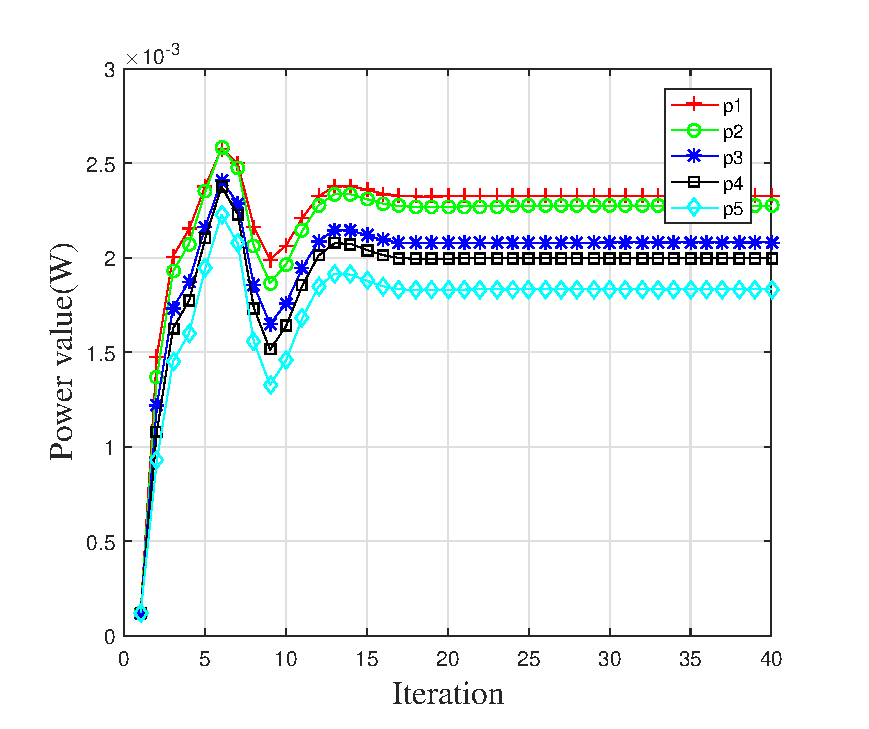
\includegraphics[width=7cm]{figures//pp.eps}
\caption{Power convergence performance.}
\label{F2}
\end{figure}
\begin{figure}[H]
\centering
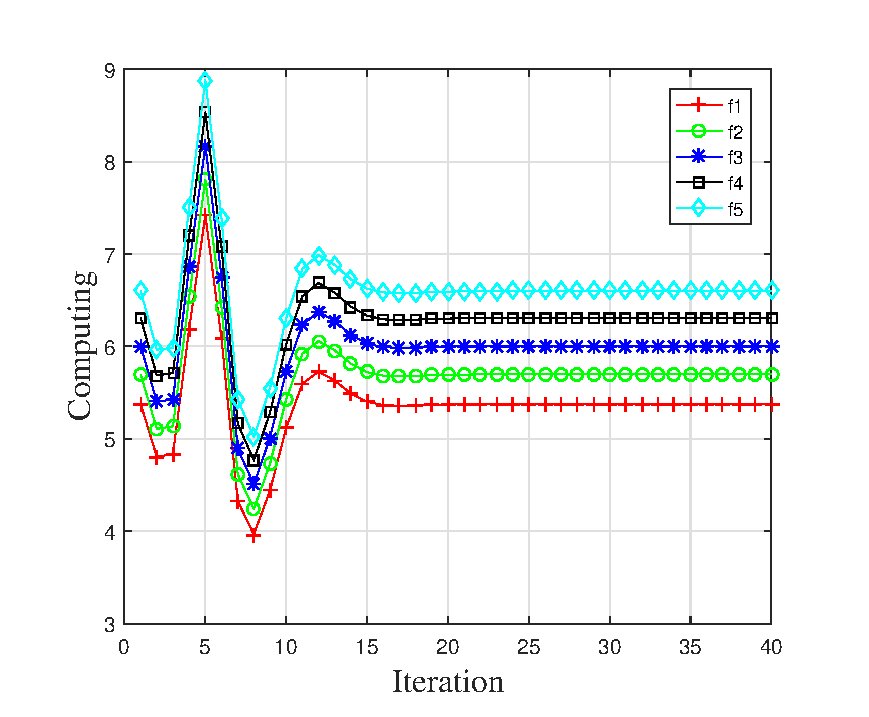
\includegraphics[width=7cm]{figures//ff.eps}
\caption{Computational resource of cloud allocation to RSU.}
\label{F3}
\end{figure}
\begin{figure}[H]
\centering
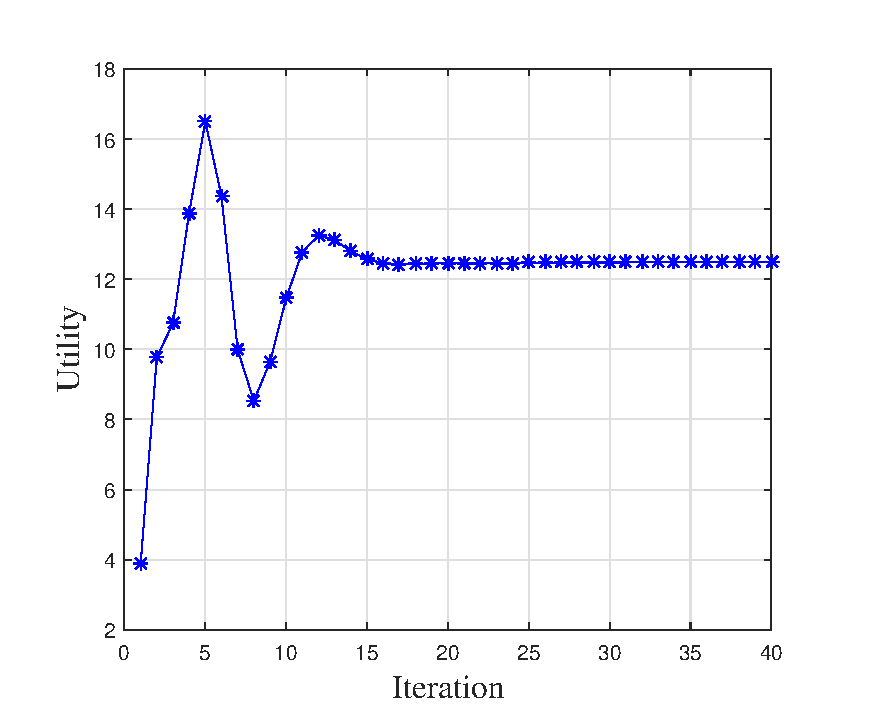
\includegraphics[width=7cm]{figures//ee.eps}
\caption{Convergence of average system utility.}
\label{F4}
\end{figure}

Fig. \ref{F2} and Fig. \ref{F3} show the power allocation of each vehicle transmitter and the corresponding computing resources allocated to the RSU in Algorithm~\ref{alg:algorithm1}, respectively. The figures show that the computing resources allocated in the cloud peak at the fifth iteration and begin to decline since the limitation of the total computing resources $f_{total}$ from the cloud is reached. The corresponding power resource allocation also changes due to computing resource allocation of robust power control and task offloading scheduling.

Fig. \ref{F4} shows the convergence of the total utility of the system when joint optimization is performed. The figure shows the convergence trend of the total utility of the network system related to power allocation and computing rate allocation. It is reasonable to observe this phenomenon because of the definition of $U$ as given in equation \eqref{E12}. $R_i$ increases logarithmically as the power vector $\mathbf{p}$ increases, resulting in diminishing marginal returns. Therefore, as the number of iterations increases, the incremental increase in utility value becomes smaller and smaller, eventually leading to a plateau in utility value. The upload time $t_{i,up}$, the denominator of $U$, decreases when the power vector $\mathbf{p}$ decreases. As the computing power vector $\mathbf{f}$ increases, the executive utility of the numerator part, $t_{i,exe}$, decreases inversely proportional. However, the numerator increases with the increase of vector $\mathbf{f}$.

In the MEC-Enabled vehicular cloud system, it is necessary to take into account the vehicle mobility. Next, we explored how the movement of vehicles affects system performance. We assumed that any changes in vehicle speed during the designated time period are insignificant. In order to further clarify the influence of speed-induced Doppler shift on system performance, the comparison between the benchmark value and the increasing speed measurement is simulated under the condition of constant vehicle speed in the system.

Fig. \ref{F5} illustrates the effect of different speeds on system performance in a highly mobile
vehicular environment. Since the relative speed in the V2R link is zero and the speed of all vehicles in the same network, there is no Doppler effect. The vehicle speed during communication is set to 20 m/s, 30 m/s, 40 m/s, 50 m/s, and 60 m/s. As shown in Figure \ref{F5}, the utility value of the vehicular network experiences a decrease as the vehicle speed increases. This is because a higher speed causes an increased Doppler frequency shift within the network, which in turn causes greater channel uncertainty and a subsequent decrease in utility.
%The result also proves that methods tend to obtain better utility when the vehicle speed is low.
\begin{figure}[H]
\centering
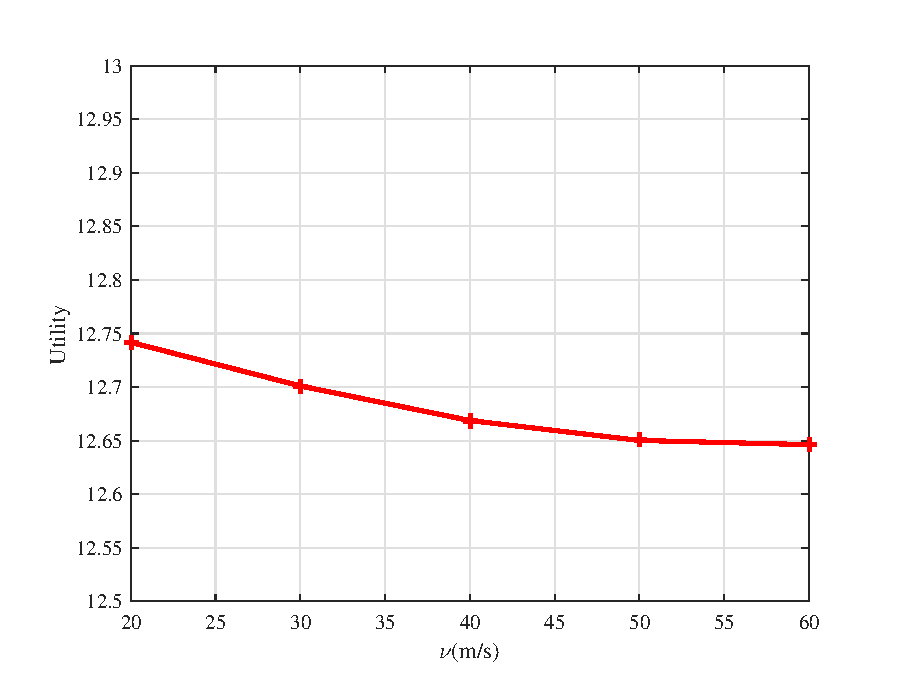
\includegraphics[width=7cm]{figures//diffspeed1.eps}
\caption{Comparison of average system utilities with different speeds.}
\label{F5}
\end{figure}

After considering the vehicle mobility, the performance of the proposed scheme is further verified. Fig. \ref{F6} shows the effect of the same and different speeds of each vehicle when different $\varepsilon_1$ is used on the total utility. The figure shows that the system utility changes when $\varepsilon_1$ changes. The utility of each vehicle at different speeds is higher than that of all vehicles at the same speed. This result characterizes the high robustness of the proposed method when implemented in complex dynamic vehicle networks.
\begin{figure}[H]
\centering
\includegraphics[width=7cm]{figures//diff_e1.eps}
\caption{Comparison of average system utility with different $\varepsilon_1$.}
\label{F6}
\end{figure}

For the computation rate allocation, we choose the default task input size as $d_u=420KB$ (which can be referred to \cite{Xu2015}), We evaluate the system utility performance with different benchmark schemes. It tries to show the convergence performance of our proposed algorithm. Simulation results try to show that the proposed method is better than the three benchmark schemes. The benchmark schemes are described as follows
\begin{itemize}
\item[1)]``Independently offloading and power control'' (denoted as ``IOP''), the vehicles independently perform  power control and computing rate allocation without the optimal value for each other.
\item[2)]``��Without vehicle power control''(denoted as ``Without-VPC''), the transmit power of the vehicles is set as the average power during the offloading.
\item[3)]``��Without computing rate allocation'' (denoted as ``Without-CRA''), the computing rate allocation of the cloud is set as a fixed value during the offloading.
    %Similar to [?]Jiang2016  Similar to: \cite{Jiang2016},
\end{itemize}

Fig. \ref{F7} shows the iterative convergence of the total utility of the system in different cases, and the figure that shows the robust joint optimization performance is better than the other three schemes. The figure show that the four methods converge to a stable value in the late iteration and the performance of proposed scheme is the best.

In order to reflect a more realistic situation, the CPU task lode (Megzcycles) required for each vehicle are often different, therefore we set the CPU task load (Megzcycles) of the five vehicles to 1600, 1700, 1800, 1900 and 2000.
\begin{figure}[H]
\centering
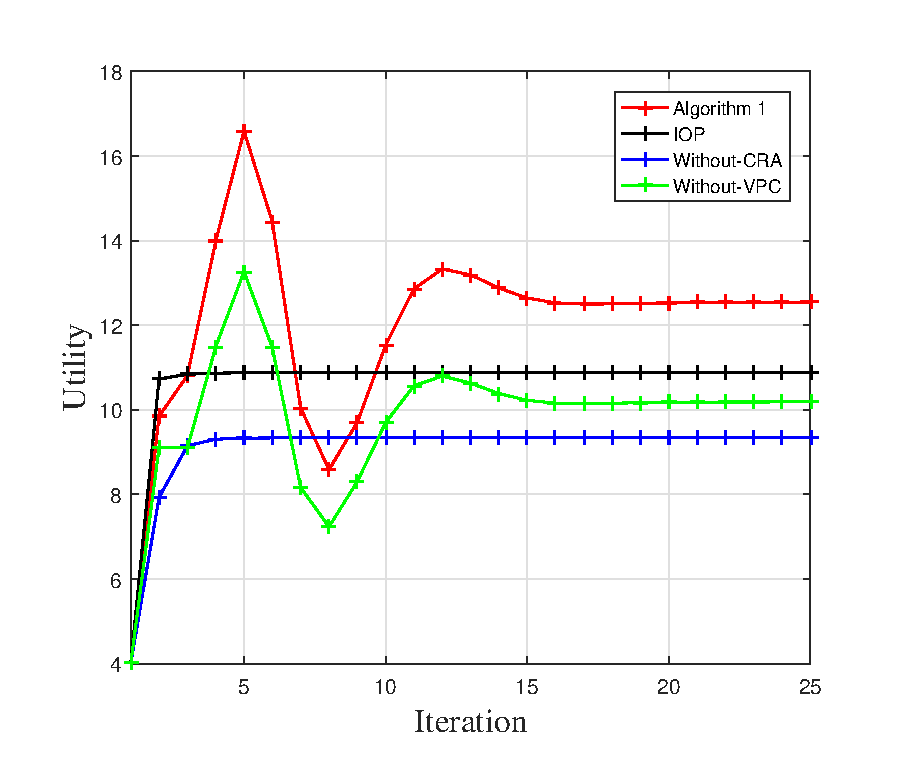
\includegraphics[width=7cm]{figures//compare.eps}
\caption{System utility convergence for different methods.}
\label{F7}
\end{figure}

In Fig. \ref{F7}, with the increase of the iteration number, the average system utility of vehicles changes gradually and tends to be stable. In the independent optimization process, the computational  rate allocation is performed first, and the optimal power allocation is not known at this time. The power and computing rate alternate optimization method is used, and the corresponding optimal value can be obtained for each iteration. Individual optimization first optimizes the power vector $\mathbf{p}$. After the result is obtained, the result is used to optimize of computational rate allocation, and then the computing rate are optimized, the system is obtained. However, if joint optimization is used, then both variables can achieve the optimal value if the joint optimization is used.

The average system utility of the four competing schemes is plotted in Fig. \ref{F8} with different task input sizes $d_u$. The figure shows that the average system utilities of all schemes decrease as the task input sizes increase. The figure also shows that the performance gains of the other schemes also have a similar trend.
This phenomenon is reasonable, since the definition of $U$ in \eqref{E12} shows that the increase in workload has a negative impact on the system performance.
\begin{figure}[H]
\centering
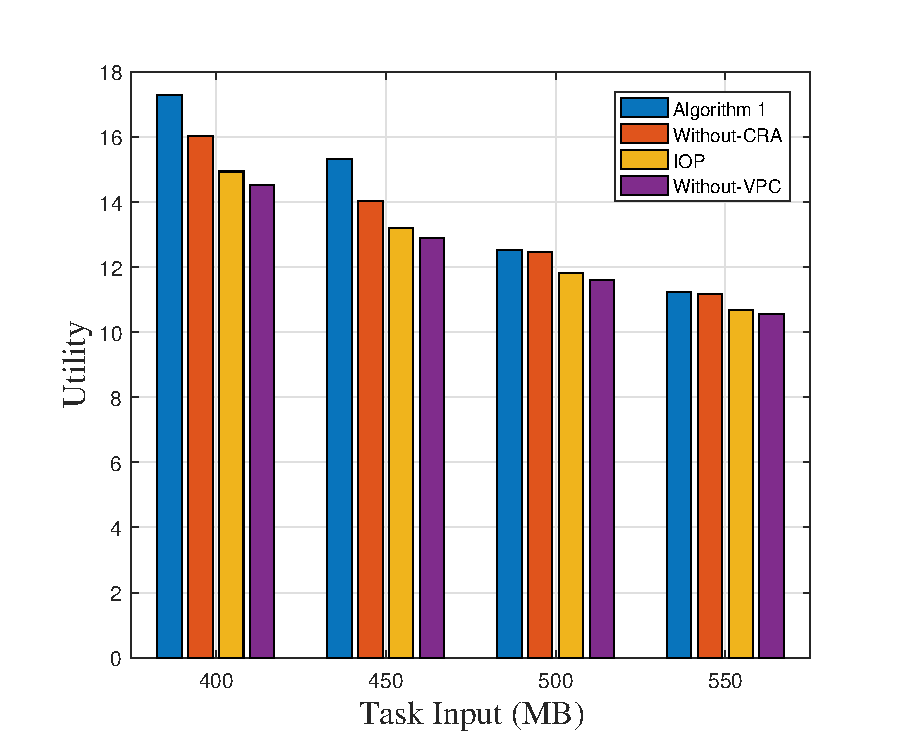
\includegraphics[width=7cm]{figures//diff_dup.eps}
\caption{Comparison of average system utility with different task input sizes $d_u$.}
\label{F8}
\end{figure}
\begin{figure}[H]
\centering
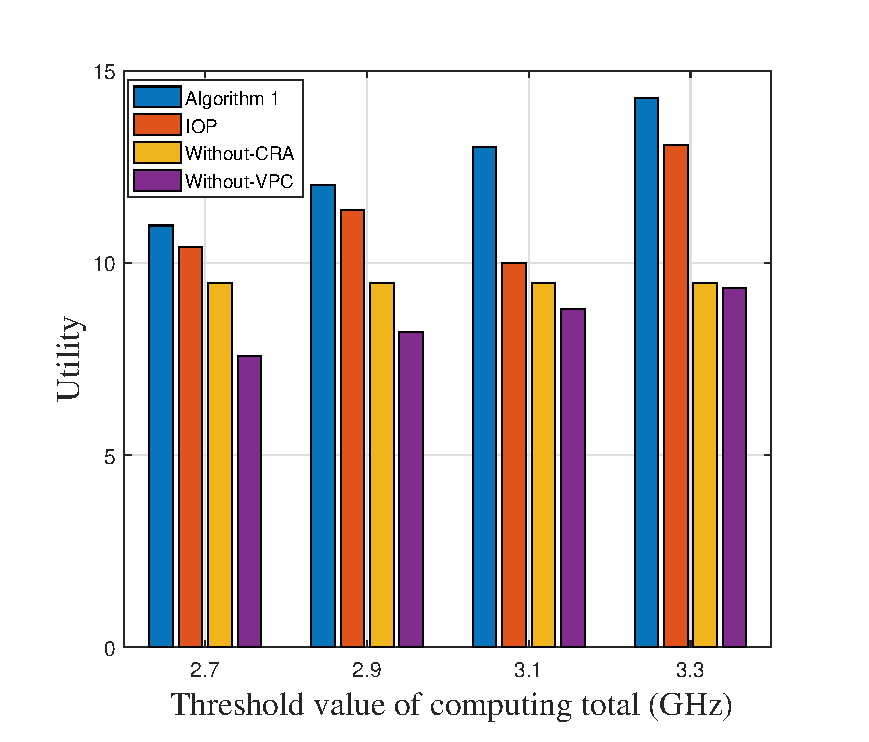
\includegraphics[width=7cm]{figures//diff_total.eps}
\caption{Comparison for average system utility with different $f_{total}$.}
\label{F9}
\end{figure}
\begin{figure}[H]
\centering
\includegraphics[width=7cm]{figures//diff_c.eps}
\caption{Comparison of average system utility with different task workloads $c_{i,e}$.}
\label{F10}
\end{figure}

Fig. \ref{F9} shows the total system cost comparisons with different $f_{total}$. The system utility is small when the computational capability is small, since the computational capability in the cloud is limited.
It is found that in Fig. \ref{F10} the system utility tends to decrease when the data size increases. This is because the computational tasks require more upload time when the data sizes are larger.
\section{Conclusions}\label{Conclusions}
In this paper, we investigated a novel approach to robust power control and task offloading for cloud-assisted MEC in vehicular networks. The optimization scheme aims to guarantee the vehicle's QoS is maintained while maximizing utility. Since channel uncertainty exists, the optimization is constrained by transmission rate, computational communication latency, and probability forms of co-channel interference. The original optimization problem is formulated as a robust power control and task offloading scheduling problem, which is very difficult to solve. The SCA technique is applied to transform the NP-hard problem of variable coupling into a treatable convex problem. The robust power control and task offloading scheduling algorithm is used to develop feasible solutions. Simulation results showed that our proposed algorithm obtains solutions that approximate the optima. Significant improvement in terms of average system offloading utilities can be achieved, compared to the existing approaches.

%\section*{Acknowledgment}
%This work is supported partly by National Natural Science Foundation of China under Grant 62273298, 62273295.

\bibliography{./reference/reference}
\bibliographystyle{IEEEtran}
%\bibliographystyle{plainnat}
%\bibliographystyle{unsrtnat}
\end{document}
